\documentclass[11pt,a4paper]{article}\usepackage[utf8]{inputenc}

\usepackage[T1]{fontenc}
\usepackage{tgpagella}
\usepackage[spanish]{babel}
\usepackage{geometry}
\usepackage{graphicx}
\usepackage{booktabs}
\usepackage{array}
\usepackage{xcolor}
\usepackage{titlesec}
\usepackage{fancyhdr}
\usepackage[parfill]{parskip}
\usepackage[expansion=false]{microtype}
\usepackage{hyperref}
\usepackage{setspace}
\usepackage{needspace}

\geometry{top=3.0cm,bottom=3.0cm,left=3.5cm,right=3.5cm}
\setlength{\parskip}{0.65em}
\setlength{\parindent}{0em}

\definecolor{azulai}{RGB}{30,80,140}
\definecolor{doradoai}{RGB}{140,90,0}
\definecolor{grisai}{RGB}{70,70,70}

\titleformat{\section}{\Large\bfseries\color{azulai}}{}{0em}{}[{\color{azulai}\titlerule[0.5pt]\nopagebreak[4]}]
\titlespacing*{\section}{0pt}{1.8em}{0.8em}
\titleformat{\subsection}{\large\bfseries\color{doradoai}}{}{0em}{}[{\nopagebreak[4]}]
\titlespacing*{\subsection}{0pt}{1.4em}{0.5em}
\titleformat{\subsubsection}{\normalsize\bfseries\color{grisai}}{}{0em}{}[{\nopagebreak[4]}]
\titlespacing*{\subsubsection}{0pt}{1.0em}{0.3em}

\pagestyle{fancy}\fancyhf{}
\rhead{\textcolor{grisai}{\small Virginia Riezu — Arquitectura Interna}}
\lhead{\textcolor{grisai}{\small Carta Natal Completa}}
\cfoot{\textcolor{grisai}{\small\thepage}}
\renewcommand{\headrulewidth}{0.3pt}

\hypersetup{colorlinks=true,linkcolor=azulai,urlcolor=azulai}
\setstretch{1.45}
\tolerance=1500
\emergencystretch=4em

\begin{document}

% ── Portada ──────────────────────────────────────────────────────────────────
\begin{titlepage}
  \centering
  \vspace*{1.5cm}
  {\Huge\bfseries\color{azulai} Carta Natal Completa}\\[0.5cm]
  {\large\color{grisai} Arquitectura Interna}\\[0.3cm]
  {\small\itshape\color{grisai} Un método para sostener cuerpo, energía y vida con coherencia}\\[2cm]
  {\huge\color{doradoai} Virginia Riezu}\\[1.5cm]
  {\Large 06/09/1975 \quad 01:30}\\[0.3cm]
  {\Large Pamplona, España}\\[0.3cm]
  {\normalsize Lat: 42.8157° \quad Lon: -1.6522° \quad UTC+02:00}\\[0.3cm]
  {\normalsize Ascendente: Géminis 29°04' \quad
    MC: Piscis 3°22'}\\[2.5cm]
  \vfill
  {\small Generado el 09/05/2026}
\end{titlepage}

\tableofcontents
\newpage

% ── Rueda ─────────────────────────────────────────────────────────────────────
\section{Carta Natal}
\begin{figure}[h!]
  \centering
  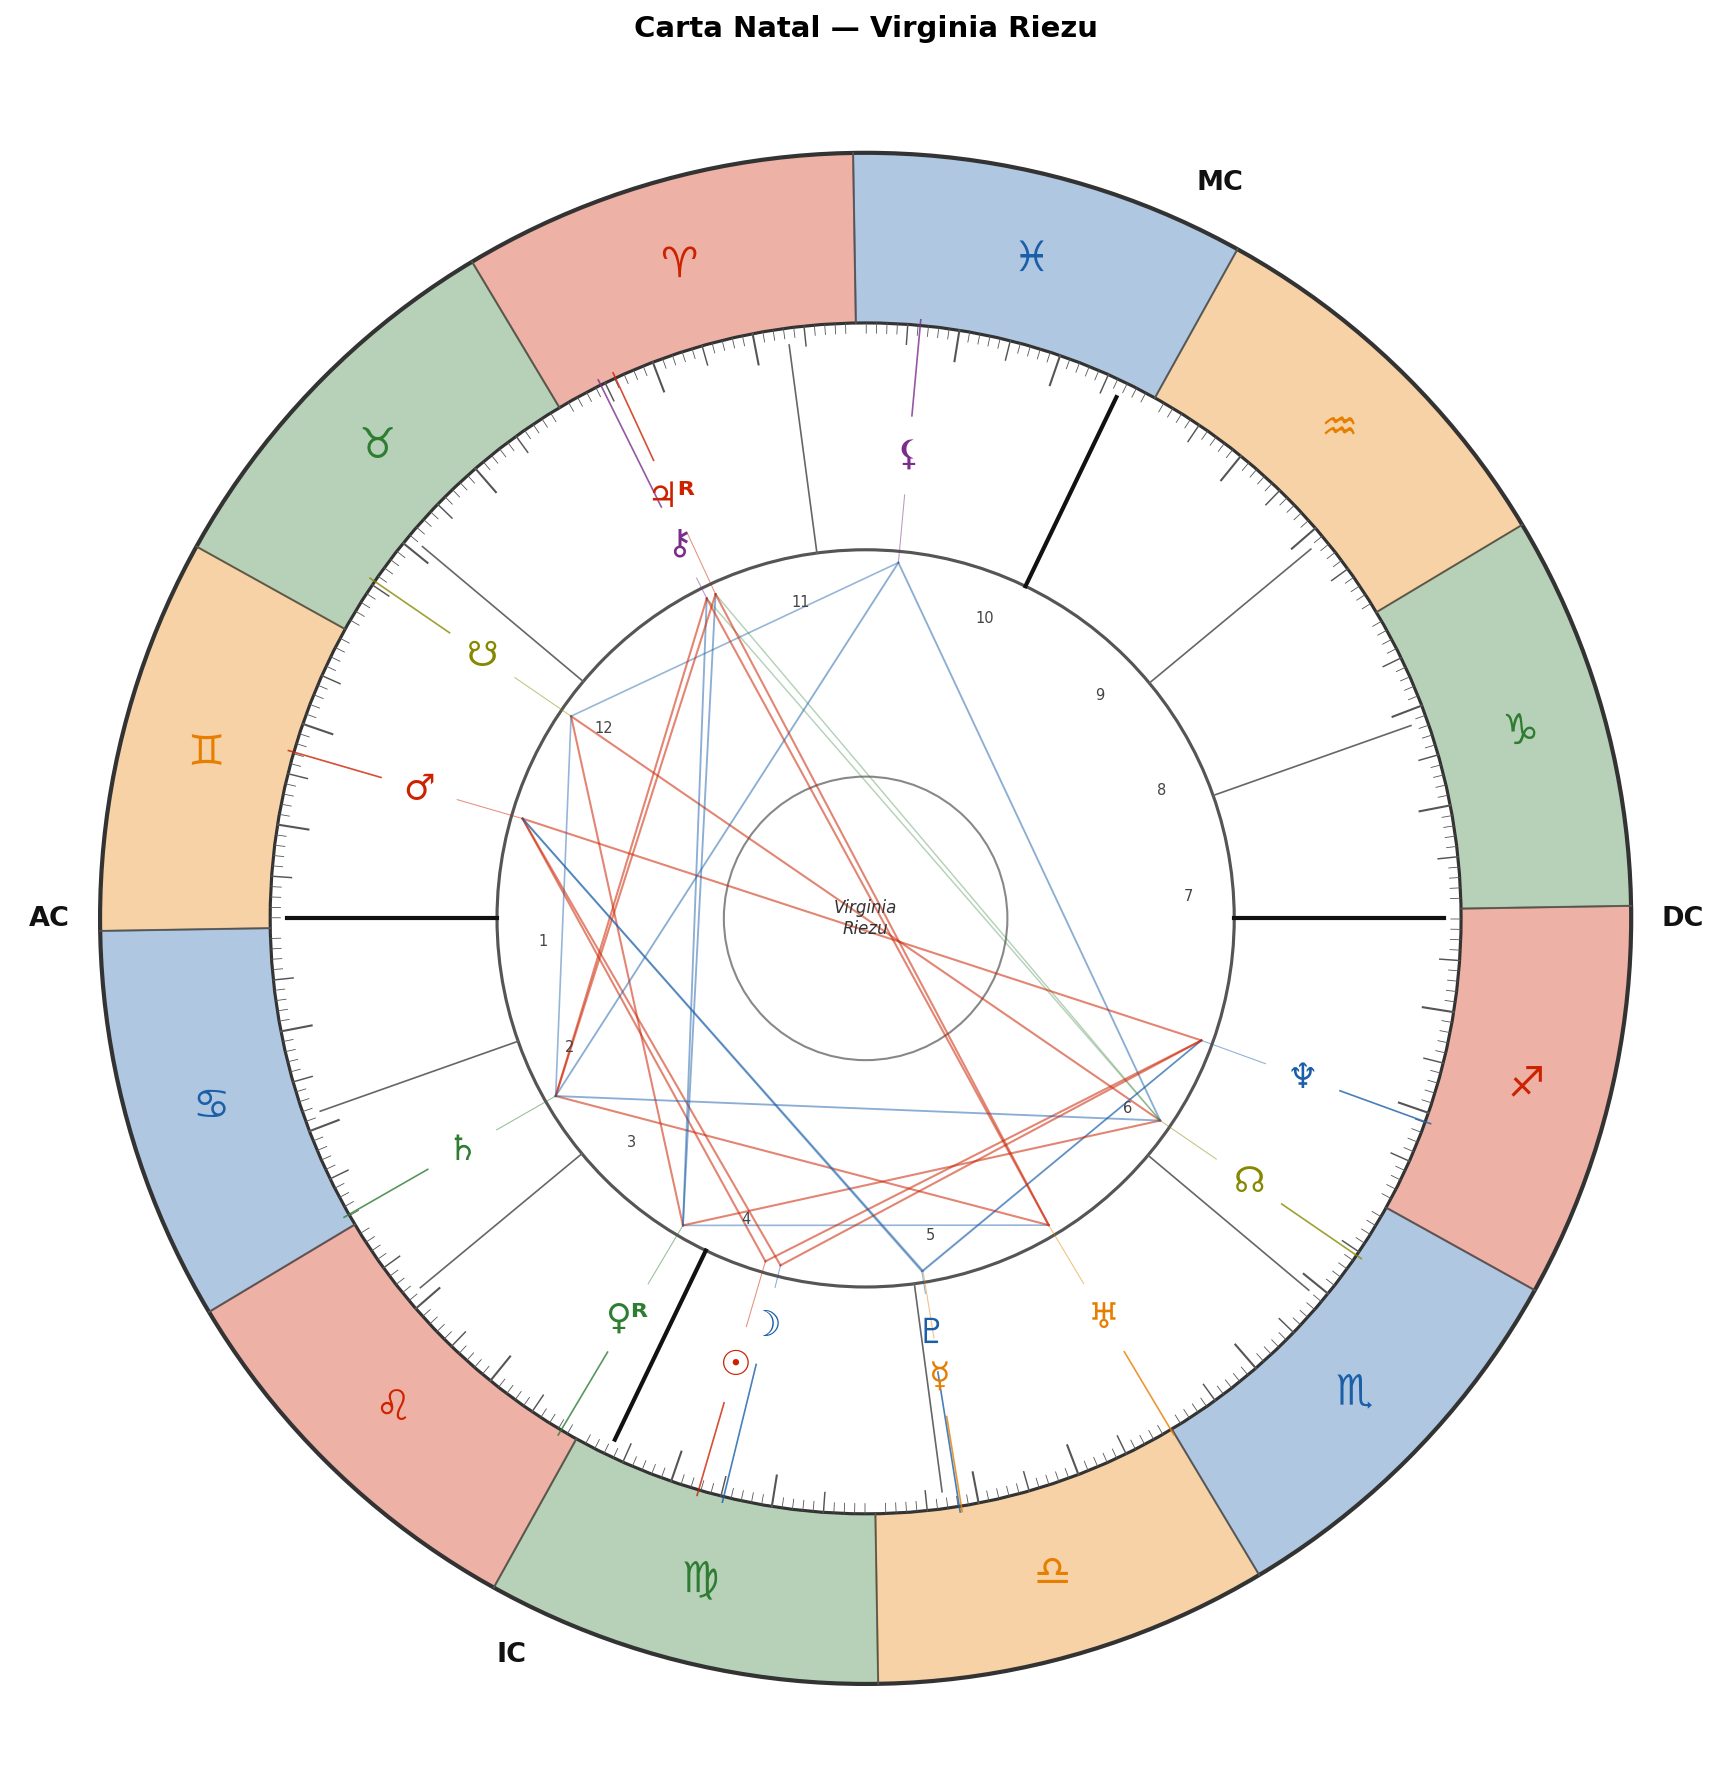
\includegraphics[width=0.90\textwidth]{Virginia_Riezu_AI_rueda.png}
  \caption{Carta natal de Virginia Riezu — 06/09/1975 01:30 — Pamplona, España}
\end{figure}

\newpage

% ── Tabla de posiciones ───────────────────────────────────────────────────────
\section{Posiciones Planetarias}

\begin{center}
\begin{tabular}{llrrlll}
  \toprule
  \textbf{Planeta} & \textbf{Signo} & \textbf{Grado} & \textbf{Casa} &
  \textbf{Elemento} & \textbf{R} \\
  \midrule
  Sol & Virgo & 12°46' & 4 & Tierra &  \\
  Luna & Virgo & 15°17' & 4 & Tierra &  \\
  Mercurio & Libra & 8°18' & 5 & Aire &  \\
  Venus & Leo & 28°18' & 3 & Fuego & R \\
  Marte & Géminis & 12°51' & 12 & Aire &  \\
  Júpiter & Aries & 23°54' & 11 & Fuego & R \\
  Saturno & Cáncer & 28°53' & 2 & Agua &  \\
  Urano & Libra & 29°54' & 5 & Aire &  \\
  Neptuno & Sagitario & 9°05' & 6 & Fuego &  \\
  Plutón & Libra & 8°07' & 5 & Aire &  \\
  Quirón & Aries & 25°28' & 11 & Fuego &  \\
  Lilith & Piscis & 23°48' & 10 & Agua &  \\
  Nodo Norte & Escorpio & 24°36' & 6 & Agua &  \\
  Nodo Sur & Tauro & 24°36' & 12 & Tierra &  \\
  \bottomrule
\end{tabular}
\end{center}

\vspace{0.5cm}
\begin{itemize}
  \item \textbf{Ascendente:} Géminis 29°04'
  \item \textbf{Medio Cielo:} Piscis 3°22'
\end{itemize}

\newpage

% ── Interpretación ────────────────────────────────────────────────────────────
\section{Interpretación — Arquitectura Interna}

\begin{center}
{\small\itshape
No se trata de definirte. Se trata de observar cómo se organiza tu energía,\
dónde puedes perder equilibrio y qué apoyos te ayudan a sostenerte.
}
\end{center}

\vspace{0.5cm}

\subsection{1. Visión General}

Tu carta muestra la siguiente distribución de elementos: Fuego 3.5, Tierra 4, Aire 8, Agua 1. Aire (desapego, análisis, pensamiento relacional y capacidad de perspectiva): ahí está el peso de tu carta. Es el registro desde el que tu energía se activa con más fluidez y sin esfuerzo consciente. Agua (profundidad emocional, capacidad de resonancia, sensibilidad abierta) está poco representado en tu carta. Ese territorio puede pedirte un esfuerzo consciente, especialmente cuando la presión sube.  Tu Medio Cielo en Piscis: La creatividad, la sensibilidad hacia el entorno y la capacidad de adaptarte a distintos contextos humanos. Funcionas bien en espacios donde hace falta imaginación, escucha o flexibilidad.

\subsection{2. Ejes Principales}

\subsubsection*{Sol en Virgo — Casa 4}
Tu Sol en Virgo construye tu identidad a través del análisis, la mejora y la utilidad práctica. Tu energía se activa cuando hay algo concreto que ordenar, mejorar o entender bien. El rigor y la competencia son tus formas de afirmarte. El riesgo es el perfeccionismo: la autoexigencia puede volverse más dura que el error que intenta corregir. En Casa 4, necesitas una base emocional estable desde la que moverte. La sensación de hogar, intimidad y protección tiene mucho peso en cómo te desarrollas. Sueles necesitar espacios donde bajar la guardia y sentir que no tienes que sostener nada hacia afuera constantemente. Cuando esa base falta, el desgaste aparece aunque externamente todo parezca funcionar.

\subsubsection*{Luna en Virgo — Casa 4}
Tu Luna en Virgo procesa las emociones a través del análisis y la búsqueda de orden. Sueles observar y evaluar constantemente cómo estás. Eso puede ser útil o puede convertirse en un obstáculo cuando la emoción necesita ser sentida antes de ser analizada. La claridad en el entorno cotidiano y la sensación de utilidad funcionan como suelo. En Casa 4, lo emocional tiene mucha relación con el hogar, la intimidad y la sensación de protección. El entorno cercano influye profundamente en cómo te sientes y en la capacidad de descansar de verdad. Cuando la base emocional o doméstica es inestable, el desgaste suele aparecer rápidamente aunque intentes seguir funcionando.

\subsubsection*{Ascendente Géminis}
Tu Ascendente en Géminis hace que te muestres al mundo como una persona ágil, curiosa y comunicativa. Entras al entorno con preguntas y conexiones. Puede haber una brecha entre esta ligereza aparente y la profundidad de lo que realmente sientes o piensas. Su regente es Mercurio, en Libra y Casa 5. El Ascendente toma el tono de Libra: armoniosa, diplomática y cuidadosa en el trato. Esa energía opera principalmente desde la creatividad, la expresión personal y la capacidad de disfrutar.

\subsubsection*{Grados finales de signo}
Los grados finales de signo muestran funciones que están cerca de un punto de cierre, maduración o cambio de modo. No se interpretan como destino ni como algo negativo, sino como zonas donde la energía del signo aparece muy concentrada. Puede haber más intensidad, menos margen para funcionar de forma automática y una sensación interna de que una forma antigua de responder ya no se sostiene igual.

En esta carta hay posiciones en grado anarético. El grado 29 suele señalar una función llevada al límite de su signo: hay mucha experiencia acumulada, pero también una presión interna para dejar de repetir el patrón de forma inconsciente.

Urano en Libra 29°54', Casa 5 aparece en grado anarético. La necesidad de libertad, cambio y ruptura de patrones aparece en un punto de máxima intensidad. Puede haber muy poca tolerancia a estructuras que se sienten cerradas, rígidas o demasiado previsibles. Cuando algo limita la autenticidad o el movimiento interno, la desconexión puede aparecer de forma repentina. El reto está en no convertir cada sensación de encierro en ruptura inmediata, sino en crear espacio antes de llegar al corte.

Ascendente en Géminis 29°04' aparece en grado anarético. Esto intensifica la forma en que entras en la vida y respondes al entorno. No se vive como un Ascendente en Géminis simple o ligero, sino como una función muy activada: hay necesidad de responder, adaptarte, leer el contexto y encontrar una forma de colocarte en el mundo. Puede haber sensación de urgencia identitaria, como si no bastara con ser de una sola manera. El cuerpo puede vivir el entorno con mucha rapidez, y por eso la regulación necesita pausa antes de reaccionar automáticamente.

Descendente en Sagitario 29°04' aparece en grado anarético. Esto lleva mucha intensidad al territorio vincular. Las relaciones no suelen sentirse neutras: activan crecimiento, contraste, necesidad de verdad y revisión de la forma de vincularte. Puede haber encuentros que funcionan como aceleradores de consciencia, porque muestran con mucha claridad dónde hay dependencia, expectativa o necesidad de libertad. El aprendizaje está en no vivir el vínculo como algo que obliga a perder centro, sino como un espacio donde la relación también necesita estructura interna.

También aparecen posiciones en grado previo al anarético. No tienen la misma presión que el grado 29, pero sí muestran zonas donde ya existe mucha maduración acumulada y cierta necesidad de revisar cómo se está usando esa energía.

Venus en Leo 28°18', Casa 3 aparece en grado previo al anarético. La forma de vincularte, desear, cuidar y buscar armonía aparece muy intensificada. No suele bastar con vínculos tibios, afectos ambiguos o entornos sin belleza ni calidez real. Puede haber cansancio de adaptarte afectivamente o de sostener formas de relación que ya no alimentan la vitalidad. El aprendizaje está en reconocer qué vínculos, espacios y elecciones tienen vida real para ti.

Saturno en Cáncer 28°53', Casa 2 aparece en grado previo al anarético. La estructura, la responsabilidad y el límite aparecen muy intensificados. Puede haber una gran capacidad para sostener, resistir y hacerse cargo, pero también cansancio profundo de funcionar desde exigencia. El sistema puede seguir adelante incluso cuando el cuerpo ya está pidiendo pausa. El aprendizaje está en comprender que parar también forma parte de la estructura, no es una pérdida de control.

Cuando varios puntos de la carta se sitúan al final de signo, la interpretación necesita considerar que el sistema puede funcionar con menos margen de regulación automática. No significa que haya más dificultad, sino que esas zonas piden más cuerpo, más pausa y más consciencia antes de seguir respondiendo desde el patrón habitual.



\subsection{3. Organización de la Energía}

Tu Mercurio en Libra piensa teniendo en cuenta varias posiciones a la vez. Puedes ver con facilidad lo que cada parte necesita o defiende. El riesgo aparece cuando considerar demasiadas opciones retrasa una decisión que ya necesita tomarse. En Casa 5, la mente necesita creatividad, expresión y cierta libertad para funcionar bien. Piensas mejor cuando hay entusiasmo, juego o posibilidad de poner algo personal en lo que haces. Tu Venus en Leo necesita expresión, reconocimiento y cierta alegría compartida en el vínculo. El afecto se activa cuando puedes mostrarte y sentir una respuesta cálida. El riesgo aparece cuando la falta de reconocimiento se vive como falta de amor. En Casa 3, el afecto fluye especialmente a través de la conversación, la cercanía y el intercambio cotidiano. La comunicación tiene mucho peso en cómo se construyen tus relaciones. Tu Marte en Géminis actúa a través de la palabra, las ideas y la movilidad. Puedes hacer varias cosas a la vez y reaccionar rápido ante estímulos distintos. El riesgo aparece cuando hay demasiadas direcciones abiertas y la energía se dispersa. En Casa 12, gran parte de la energía funciona de forma interna o poco visible desde fuera. Necesitas momentos de retirada, silencio o trabajo en soledad para ordenar bien el impulso antes de actuar.

\subsection{4. Estructura y Tensión}

\subsubsection*{Concentración de energía}

Hay una concentración notable en Casa 5: Mercurio, Urano y Plutón. Cuando varios planetas ocupan la misma casa, esa área absorbe buena parte de la actividad vital. En esta carta, el foco de la creatividad, el disfrute y la expresión personal funciona como núcleo central: ahí se acumula la presión, la demanda es mayor y también hay más recursos disponibles para operar. No es necesariamente un conflicto, pero sí un punto de alta intensidad sostenida.



Los aspectos aparecen organizados en dos niveles. Los aspectos exactos (orbe igual o menor a 1°) suelen sentirse de forma más inmediata y constante en la vida cotidiana. Los aspectos estructurales tienen un orbe más amplio, pero siguen describiendo dinámicas importantes que se repiten a lo largo de la vida.



\Needspace{8\baselineskip}
\subsubsection*{Aspectos exactos}
No aparecen aspectos exactos especialmente fuertes dentro del orbe definido para esta lectura. Eso no significa ausencia de tensión o profundidad, sino que gran parte de las dinámicas importantes de la carta se construyen de forma más amplia y progresiva. En este caso, cobran más importancia los aspectos estructurales y la combinación general de posiciones.

\Needspace{8\baselineskip}
\subsubsection*{Aspectos estructurales}
\Needspace{7\baselineskip}
\subsubsection*{Luna (Casa 4) cuadratura Marte (Casa 12) --- orbe 2.43\textdegree}
La cuadratura Luna-Marte puede generar reacciones rápidas cuando algo te afecta. La emoción y el impulso se activan casi al mismo tiempo, y a veces actúas antes de tener claro qué necesitas. Te ayuda separar unos segundos la reacción de la acción para no convertir una emoción pasajera en un conflicto mayor.



\subsection{5. Sostén y Equilibrio}

Tu Quirón en Aries, Casa 11, señala una zona sensible relacionada con la iniciativa propia, la capacidad de afirmarte y el derecho a ocupar espacio. Puede que en algún momento hayas sentido que actuar, decidir o ir primero generaba conflicto o rechazo. Esto suele notarse especialmente en la pertenencia a grupos y los proyectos compartidos. No significa que tengas límites en ese terreno, pero sí que probablemente necesites más tiempo, cuidado o consciencia para sentir estabilidad ahí.

\vspace{0.3cm}
Tu Nodo Sur en Tauro, Casa 12, muestra una tendencia a moverte desde la necesidad de mantener estabilidad incluso cuando una situación ya necesita cambiar, especialmente en la vida privada, la necesidad de retiro y lo que cuesta mostrar directamente. Suele ser una forma de funcionar conocida o automática para ti. Tu Nodo Norte en Escorpio, Casa 6, señala la necesidad de desarrollar atravesar cambios importantes sin quedarte solo en lo conocido o controlable, especialmente en los hábitos, el trabajo cotidiano y la relación con el cuerpo. No se trata de rechazar lo anterior, sino de ampliar tu forma habitual de responder.

\vspace{0.3cm}
En tu carta hay poca presencia de Agua. Cuando aparece saturación, bloqueo o sensación de desorganización interna, suele ayudarte volver a espacios relacionados con la intimidad, el descanso emocional y los espacios donde puedes sentir sin presión. Eso puede darte más estabilidad y ayudarte a recuperar claridad.

\subsection{6. Orientación}

\subsubsection*{Qué observar}
Tu Ascendente en Géminis describe la forma en que otras personas suelen percibirte al principio. Eso no siempre coincide con cómo vives las cosas internamente o con las tensiones más importantes de tu carta. Cuando hay demasiada distancia entre lo que muestras y lo que realmente te ocurre, aparece desgaste.

\subsubsection*{Qué puede desestabilizar}
Hay ciertas tensiones en tu carta que pueden activarse con bastante fuerza: Nodo Norte-Nodo Sur, Sol-Marte, Júpiter-Nodo Norte. Cuando varias coinciden al mismo tiempo, puede aparecer sensación de saturación, reacción excesiva o dificultad para mantener claridad.

\subsubsection*{Qué estructura y sostiene}
Tu Sol en Virgo, Casa 4, muestra un terreno importante de estabilidad para ti. Cuando tu forma de actuar está alineada con lo que realmente valoras, suele aparecer más claridad y menos dispersión.

\subsubsection*{Orientación práctica}
Una orientación práctica: en tu carta hay poca Agua. A veces puedes seguir funcionando aunque lleves tiempo acumulando cansancio emocional. Parar, descansar de verdad o permitirte sentir antes de seguir avanzando puede ayudarte a no endurecerte demasiado.

\vspace{1cm}
\begin{center}
{\small\itshape\color{grisai}
La astrología se usa aquí como lenguaje simbólico de observación, no como una definición de quién eres.\\
Esta interpretación es tu mapa de posibilidades, no tu destino fijo.
}
\end{center}

\end{document}
